\newpage
\section{Open-loop System}

\subsection{System Model}

The chemical process illustrated in Figure~\ref{fig:reactor_scheme} represents an axial dispersion tubular reactor, which incorporates diffusion, convection, and a first-order irreversible chemical reaction \autocite{levenspiel1998chemical}. The reactor is equipped with a recycle mechanism, allowing a fraction of the product stream to re-enter the reactor to ensure the consumption of any unreacted substrate. By applying first-principle modeling through relevant mass balance relations on an infinitesimally small section of the reactor, the reactor's dynamics can be described by a second-order parabolic PDE, a common class of equations used to characterize diffusion-convection-reaction systems \autocite{jensen1982bifurcation}. The resulting PDE that describes the reactor model is given by:

\begin{equation} \label{eq:PDE_original_model}
    \dot{x}(\zeta, t) = D \partial_{\zeta \zeta} c(\zeta, t) - v \partial_\zeta c(\zeta, t) + k_r c(\zeta, t)
\end{equation}

subject to Dankwerts boundary conditions:

\begin{align} \label{eq:BC}
    \begin{cases}
        &D \partial_\zeta c(0, t) - v c(0, t) = -v \left[ R c(1, t-\tau) + (1-R) u(t) \right] \\
        &\partial_\zeta c(1, t) = 0 \\
        &y(t) = c(1, t)
    \end{cases}
\end{align}

Here, $c(\zeta, t)$ denotes the concentration along the reactor, representing the state of the system. The physical parameters $D$, $v$, $k_r$, $R$, and $\tau$ correspond to the diffusion coefficient, flow velocity along the reactor, reaction constant, recycle ratio, and residence time of the recycle stream, respectively. The spatial and temporal coordinates of the system are represented by $\zeta$ and $t$, where $\zeta \in [0, 1]$ and $t \in [0, \infty)$.

Dankwerts boundary conditions are particularly suitable for modeling axial tubular reactors, as they account for deviations from perfect mixing and piston flow, assuming negligible transport lags in connecting lines \autocite{danckwerts1993continuous}. These conditions make the model more realistic for chemical reactors of this type. The input and the output of the system are also present in the boundary conditions. The system output is measured at the reactor outlet, while the input is applied at the inlet. Additionally, the delayed state resulting from the recycled portion of the flow, occurring $\tau$ time units ago, is incorporated into the inlet; all as shown in Equation~\ref{eq:BC}.


\begin{figure}[ht]
    \centering
    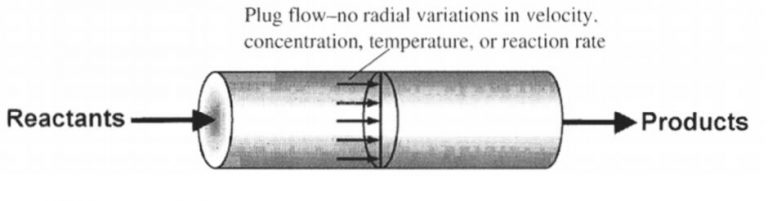
\includegraphics[width=0.7\textwidth]{Figures/sample.jpeg}
    \caption{Sample figure.}
    \label{fig:reactor_scheme}
\end{figure}

\subsection{PDE Representation of Delay Term}

One effective method for addressing delay in systems is to represent the delay using an alternative transport partial differential equation (PDE). This approach is particularly advantageous when the problem already involves similar forms of PDEs, as is the case in the current study. To specifically address the delay in the system under consideration, the state variable $c(\zeta, t)$ is expanded into a vector of functions $C(\zeta, t) \equiv [c_1(\zeta, t), c_2(\zeta, t)]^T$, where $c_1(\zeta, t)$ represents the concentration within the reactor, and $c_2(\zeta, t)$ is introduced as a new state variable to account for the concentration along the recycle stream. The delay is thus modeled as a pure transport process, wherein the first state $c_1(\zeta, t)$ is transported from the reactor outlet to the inlet, experiencing a delay of $\tau$ time units while in the recycle stream. As a result, Equations~\ref{eq:PDE_original_model}~and~\ref{eq:BC} may be re-formulated as follows:

\begin{align}
    \partial_t 
    \begin{bmatrix}
        c_1(\zeta, t) \\ c_2(\zeta,t)
    \end{bmatrix}
    =
    \begin{bmatrix}
        D \partial_{\zeta \zeta} - v \partial_\zeta + k_r && 0 \\
        0 && -\frac{1}{\tau} \partial_\zeta
    \end{bmatrix}
    \begin{bmatrix}
        c_1(\zeta, t) \\ c_2(\zeta,t)
    \end{bmatrix}\\
\begin{cases}
    D \partial_\zeta c_1(0, t) - v c_1(0, t) = -v \left[ R c_2(0, t) + (1-R) u(t) \right] \\
    \partial_\zeta c_1(1, t) = 0 \\
    c_1(1,t) = c_2(1,t) \\
    y(t) = c_1(1, t)
\end{cases}
\end{align}

With all state variables now expressed explicitly at a specific time instance $t$—in contrast to the previous representation where states at $t$ were directly involved with states at $t-\tau$—the system can be described in the standard state-space form of an infinite-dimensional linear time-invariant (LTI) system as $\dot{x} = \mathfrak{A} x$. Here, the state $x(\zeta, t) = [x_1(\zeta, t), x_2(\zeta, t)]^T$ is a vector of functions, and $\mathfrak{A}$ is a linear operator $\mathcal{L}(X)$ acting on a Hilbert space $X: L^2[0,1] \times L^2[0,1]$. The operator $\mathfrak{A}$ and its domain are defined in detail as shown in Equation~\ref{eq:operator_A}:

\begin{equation} \label{eq:operator_A}
    \begin{aligned}
        \mathfrak{A} \equiv&
        \begin{bmatrix}
            D \partial_{\zeta \zeta} - v \partial_\zeta + k_r & 0 \\
            0 & \frac{1}{\tau} \partial_\zeta
        \end{bmatrix}\\
        D(\mathfrak{A}) =& \Bigl\{ x = [x_1, x_2]^T \in X:
        x(\zeta), \partial_\zeta x(\zeta), \partial_{\zeta \zeta} x(\zeta) \quad \mathrm{a.c.},\\
        &D \partial_\zeta x_1(0) - v x_1(0) = -v \left[ R x_2(0) + (1-R) u \right],\\
        &\partial_\zeta x_1(1) = 0,
        x_1(1) = x_2(1) \Bigr\}
    \end{aligned}
\end{equation}

\subsection{Adjoint Operator}

Obtaining the adjoint operator $\mathfrak{A}^*$ is a crucial step in analyzing the system's properties, particularly its spectral characteristics. If the operator $\mathfrak{A}$ is shown to be self-adjoint (i.e., $\mathfrak{A} = \mathfrak{A}^*$), the system's eigenmodes can be suitably scaled to form an orthonormal basis for the entire function space, which greatly facilitates the analysis and solution of the system. However, even when the operator $\mathfrak{A}$ is not self-adjoint, the combined set of eigenmodes of $\mathfrak{A}$ and its adjoint $\mathfrak{A}^*$ may still form a bi-orthonormal basis for the given function space. This scenario is typical when $\mathfrak{A}$ is a Riesz-spectral operator \autocite{curtainbook}. Consequently, determining the adjoint operator $\mathfrak{A}^*$, as represented in Equation~\ref{eq:adjoint_A} is a pivotal step in the spectral analysis of the system.

\begin{equation} \label{eq:adjoint_A}
    \begin{aligned}
        \langle \mathfrak{A} \Phi, \Psi\rangle  = \langle \Phi, {\mathfrak{A}}^{*} \Psi\rangle  &\Rightarrow \\
        {\mathfrak{A}}^{*} =&
        \begin{bmatrix}
            D \partial_{\zeta \zeta} + v \partial_\zeta +k_r & 0\\
            0 & -\frac{1}{\tau} \partial_\zeta
        \end{bmatrix}\\
        D(\mathfrak{A}^*) =& \Bigl\{ y = [y_1, y_2]^T \in Y:
        y(\zeta), \partial_\zeta y(\zeta), \partial_{\zeta \zeta} y(\zeta) \quad \mathrm{a.c.},\\
        &D \partial_\zeta y_1(1) + v y_1(1) = \frac{1}{\tau} y_2(1) \\
        &R v y_1(0) = \frac{1}{\tau} y_2(0) \\
        &\partial_\zeta y_1(0) = 0 \Bigr\}
    \end{aligned}
\end{equation}

This suggests that the operator $\mathfrak{A}$ is not self-adjoint. To investigate whether $\mathfrak{A}$ is a Riesz-spectral operator, the spectra of both $\mathfrak{A}$ and $\mathfrak{A}^*$ must be determined by solving their characteristic equations, which is done in the upcoming section.

\subsection{Eigenvalue Problem}
The spectrum of both $\mathfrak{A}$ and $\mathfrak{A}^*$ shall be determined to show whether $\mathfrak{A}$ is a Riesz-spectral operator. In order to obtain the eigenvalues of the system, the eigenvalue problem shall be stated and the characteristic equation needs to be solved once obtained from the equations. Looking back at the state-space representation of the system $\dot{x}(\zeta, t) = \mathfrak{A} x(\zeta, t)$, with $\mathfrak{A}$ defined in Equation~\ref{eq:operator_A}, spatial part of $x(\zeta, t)$ may be isolated and used to demonstrate the eigenvalue problem \autocite{pdebook} as shown in Equation~\ref{eq:eig_prob}:

\begin{equation} \label{eq:eig_prob}
        \mathfrak{A} \Phi_i(\zeta) = \lambda_i \Phi_i(\zeta)
\end{equation}

where $\lambda_i \in \mathcal{C}$ is the $i^{\text{th}}$ eigenvalue of the operator $\mathfrak{A}$, with $\Phi_i(\zeta) = [\phi_{i,1}(\zeta), \phi_{i,2}(\zeta)]^T$ being its corresponding eigenfunction. Re-writing the spatial part for the system of PDEs considering the eigenvalues will give Equation~\ref{eq:eigval_calc_1} for a given $i$:

\begin{equation} \label{eq:eigval_calc_1}
    \begin{aligned}
        &\begin{cases}
            &\lambda \phi_1 = D \frac{d^2 \phi_1}{d \zeta ^2}  - v \frac{d \phi_1}{d \zeta} + k \phi_1 \\
            &\lambda \phi_2 = \frac{1}{\tau} \frac{d \phi_2}{d \zeta}
        \end{cases} \\ B.C. &\begin{cases}
            &D \left. \frac{d \phi_1}{d \zeta} \right|_{\zeta=0} - v \left. \phi_1 \right|_{\zeta=0} = - R v \left. \phi_2 \right|_{\zeta=0} \\
            &\left. \phi_1 \right|_{\zeta=1} = 0 \\
            &\left. \phi_1 \right|_{\zeta=1} = \left. \phi_2 \right|_{\zeta=1}
        \end{cases}
    \end{aligned}
\end{equation}

The goal is to obtain the set of eigenvalues. To do so, the second order derivative in the operator $\mathfrak{A}$ shall be converted in two first order derivatives to give Equation~\ref{eq:eigval_calc_2}:

\begin{equation} \label{eq:eigval_calc_2}
    \begin{aligned}
        % \begin{bmatrix}
        %     \tilde{\phi_1}, \tilde{\phi_2}, \tilde{\phi_3}
        % \end{bmatrix}^T \equiv \begin{bmatrix}
        %     \partial_\zeta \phi_1, \phi_1, \phi_2
        % \end{bmatrix}^T \Rightarrow \\
        \partial_\zeta \begin{bmatrix}
            \phi_1 \\ \partial_\zeta \phi_1 \\ \phi_2
        \end{bmatrix} = \begin{bmatrix}
            0 & 1 & 0 \\
            \frac{\lambda-k_r}{D} & \frac{v}{D} & 0 \\
            0 & 0 & \tau \lambda 
        \end{bmatrix} \begin{bmatrix}
            \phi_1 \\ \partial_\zeta \phi_1 \\ \phi_2
        \end{bmatrix}
    \end{aligned}
\end{equation}

which is a well-known system of ODEs in the form of $ \tilde{\Phi}_\zeta  = \tilde{\mathfrak{A}} \tilde{\Phi}$, with $\tilde{\Phi} \equiv [\phi_1, \partial_\zeta \phi_1, \phi_2]^T$ and $\tilde{\mathfrak{A}}$ as the $3 \times 3$ matrix shown in Equation~\ref{eq:eigval_calc_2}. The obtained system of ODEs has the solution of the form $\tilde{\Phi}(1) = e^{\tilde{\mathfrak{A}}(1-0)}\Phi(0)$. By introducing $\Lambda \equiv e^{\tilde{\mathfrak{A}}}$, Equation~\ref{eq:eigval_calc_3} may be deduced:

\begin{equation} \label{eq:eigval_calc_3}
    \begin{bmatrix}
        \phi_1 \\ \partial_\zeta \phi_1 \\ \phi_2
    \end{bmatrix}_{\zeta=1} = \begin{bmatrix}
        \Lambda_{1,1} & \Lambda_{1,2} & \Lambda_{1,3} \\
        \Lambda_{2,1} & \Lambda_{2,2} & \Lambda_{2,3} \\
        \Lambda_{3,1} & \Lambda_{3,2} & \Lambda_{3,3}
    \end{bmatrix} \begin{bmatrix}
        \phi_1 \\ \partial_\zeta \phi_1 \\ \phi_2
    \end{bmatrix}_{\zeta=0}
\end{equation}

Next, the boundary conditions may be plugged in Equation~\ref{eq:eigval_calc_3} accordingly to result a $3 \times 3$ algebraic system of equations shown in Equation~\ref{eq:eigval_calc_4}:

\begin{equation} \label{eq:eigval_calc_4}
    \begin{bmatrix}
        -v & D & Rv \\
        \Lambda_{2,1} & \Lambda_{2,2} & \Lambda_{2,3} \\
        (\Lambda_{1,1} - \Lambda_{3,1}) & (\Lambda_{1,2} - \Lambda_{3,2}) & (\Lambda_{1,3} - \Lambda_{3,3})
    \end{bmatrix} \begin{bmatrix}
        \phi_1 \\ \partial_\zeta \phi_1 \\ \phi_2
    \end{bmatrix}_{\zeta=0} = \tilde{\Lambda} \tilde{\Phi}_{\zeta = 0} = 0
\end{equation}

where $\tilde{\Lambda}$ is defined as the $3 \times 3$ matrix shown in Equation~\ref{eq:eigval_calc_4}. The system of algebraic equations shown in Equation~\ref{eq:eigval_calc_4} suggests that the matrix $\tilde{\Lambda}$ must be rank-deficient for appropriate values of $\lambda_i$. Therefore, to solve the characteristic equation means to set $det(\tilde{\Lambda}) = 0$. This will result in the set of eigenvalues of the operator $\mathfrak{A}$. Since an analytical solution may not be feasible, system parameters will be selected to enable numerical calculations. Physical parameters have been selected to reflect realistic values relevant to the application, with their corresponding values provided in Table~\ref{tab:pars}.

\begin{table}[h!]
    \centering
    \caption{Physical Parameters for the System}
    \label{tab:pars}
    \begin{tabular}{|c|c|c|}
    \hline
    \textbf{Parameter} & \textbf{Symbol} & \textbf{Value} \\ \hline
    Length             & $L$             & 10 m           \\ \hline
    Mass               & $m$             & 5 kg           \\ \hline
    Damping Coefficient & $c$            & 0.1 Ns/m       \\ \hline
    Spring Constant    & $k$             & 100 N/m        \\ \hline
    \end{tabular}
    \end{table}

The eigenvalue distribution in the complex plane is depicted in Figure [XXX], given parameters provided in Table~\ref{tab:pars}.

% Insert figure

Following the same procedure for the adjoint operator $\mathfrak{A}^*$ results in the set of adjoint eigenvalues $\lambda^*_i$. It can be analytically proven that $\forall i > 0$: $\lambda^*_i = \overline{\lambda_i}$. Therefore, the eigenvalue distribution for $\mathfrak{A}^*$ will be the same as for $\mathfrak{A}$, which is previously shown in Figure [XXX].

%explain Riesz and move towards eigfuns

\subsection{Eigenfunctions Representation}

\subsection{Open-loop (Zero-input) Response}